\documentclass[a4paper,12pt]{article}
\usepackage[russian, english]{babel}

\babelfont{rm}{Times New Roman}
\babelfont{sf}{Times New Roman}

\usepackage[hidelinks]{hyperref}
\usepackage{indentfirst}
\usepackage{listings}
\usepackage{xcolor}
\usepackage{here}
\usepackage{array}
\usepackage{multirow}
\usepackage{graphicx}
% многостраничные таблицы
\usepackage{longtable}
\usepackage[fleqn]{amsmath}
\usepackage{amssymb}
\usepackage{csvsimple}
\usepackage{caption}
\usepackage{pdfpages}
% captionof
% toprule bottomrule etc.
\usepackage{booktabs}
% side-by-side images
\usepackage{caption}
\usepackage{subcaption}
% enumerate biblio
\usepackage[nottoc,numbib]{tocbibind}
% sort alpha
\usepackage[backend=biber,sorting=none,style=ieee,citestyle=ieee]{biblatex}

\renewcommand{\lstlistingname}{Программа} % заголовок листингов кода

\usepackage{listings}

\definecolor{mauve}{rgb}{0.58,0,0.82}

\lstset{frame=shadowbox,
  rulesepcolor=\color{gray},
  language=Python,
  aboveskip=3mm,
  belowskip=3mm,
  showstringspaces=false,
  columns=flexible,
  basicstyle={\ttfamily},
  numbers=none,
  numberstyle=\color{black},
  keywordstyle=\color{blue},
  commentstyle=\color{green},
  stringstyle=\color{mauve},
  breaklines=true,
  breakatwhitespace=true,
  tabsize=3,
  xleftmargin=2em,
  framexleftmargin=2em,
  numbers=left,
  firstnumber=1,
  captionpos=b,
  extendedchars=\true,
  keepspaces=true,
  inputpath=../decision_theory,                     % директория с листингами
}


\usepackage[left=2cm,right=2cm,
top=2cm,bottom=2cm,bindingoffset=0cm]{geometry}

%% Нумерация картинок по секциям
\usepackage{chngcntr}
\counterwithin{figure}{section}
\counterwithin{table}{section}

%%Точки нумерации заголовков
\usepackage{titlesec}
\titlelabel{\thetitle.\quad}
\usepackage[dotinlabels]{titletoc}

%% Оформления подписи рисунка
\addto\captionsrussian{\renewcommand{\figurename}{Рисунок}}
\captionsetup[figure]{labelsep = period, justification=centering}

%% Подпись таблицы
\addto\captionsrussian{\renewcommand{\tablename}{Таблица}}
\captionsetup[table]{labelsep = period, justification=centering}

%% Подпись таблицы
%\DeclareCaptionFormat{hfillstart}{\hfill#1#2#3\par}
%\captionsetup[table]{format=hfillstart,labelsep=newline,justification=centering,skip=-10pt,textfont=bf}

%% Путь к каталогу с рисунками
\graphicspath{{fig/}}

%% Внесение titlepage в учёт счётчика страниц
\makeatletter
\renewenvironment{titlepage} {
 \thispagestyle{empty}
}
\makeatother


\addbibresource{refs.bib}

% magic
\makeatletter
\newcommand{\stackover}{\genfrac{.}{.}\z@{}}
\makeatother

\begin{document}	% начало документа
\selectlanguage{russian}

% Титульная страница
\begin{titlepage}	% начало титульной страницы

	\begin{center}		% выравнивание по центру

		\large Санкт-Петербургский политехнический университет Петра Великого\\
		\large Институт компьютерных наук и технологий \\
		\large Высшая школа программной инженерии\\[8cm]
		% название института, затем отступ 6см
		
		\huge Отчёт по практической работе\\[0.5cm] % название работы, затем отступ 0,5см
		\large ``Модифицированный метод сопряженных градиентов с тремя
		термами и его приложения в задаче восстановления изображений''\\[0.5cm]
		\large по дисциплине "Теория принятия решений"\\[3cm]

	\end{center}

	\begin{flushright} % выравнивание по правому краю
		\begin{minipage}{0.25\textwidth} % врезка в половину ширины текста
			\begin{flushleft} % выровнять её содержимое по левому краю

				\large\textbf{Работу выполнил:}\\
				\large Поздняков А.А.\\
				\large {Группа:} 5130904/00104\\
				
				\large \textbf{Преподаватель:}\\
				\large Черноруцкий И.Г.

			\end{flushleft}
		\end{minipage}
	\end{flushright}
	
	\vfill % заполнить всё доступное ниже пространство
	% \vspace{10\baselineskip}

	\begin{center}
	\large Санкт-Петербург\\
	\large \the\year % вывести дату
	\end{center} % закончить выравнивание по центру

\end{titlepage} % конец титульной страницы



\tableofcontents
\newpage

\section{Введение}

За основу была взята статья ``Y.Ismail Ibrahim и H.Mohammed Khudhur,“Modified
three-term conjugate gradient algorithm and its applications in image
restoration”, Indonesian Journal of Electrical Engineering and Computer Science,
т. 28, No 3, с. 1510, дек. 2022, ISSN: 2502-4752. DOI: 10.11591/ijeecs.
v28.i3.pp1510-1517. url: http://dx.doi.org/10.11591/ijeecs.v28.i3.pp1510- 1517''.

\newpage

\newpage
\nocite{*}
\printbibliography[heading=bibintoc]

\newpage
\section{Приложение}

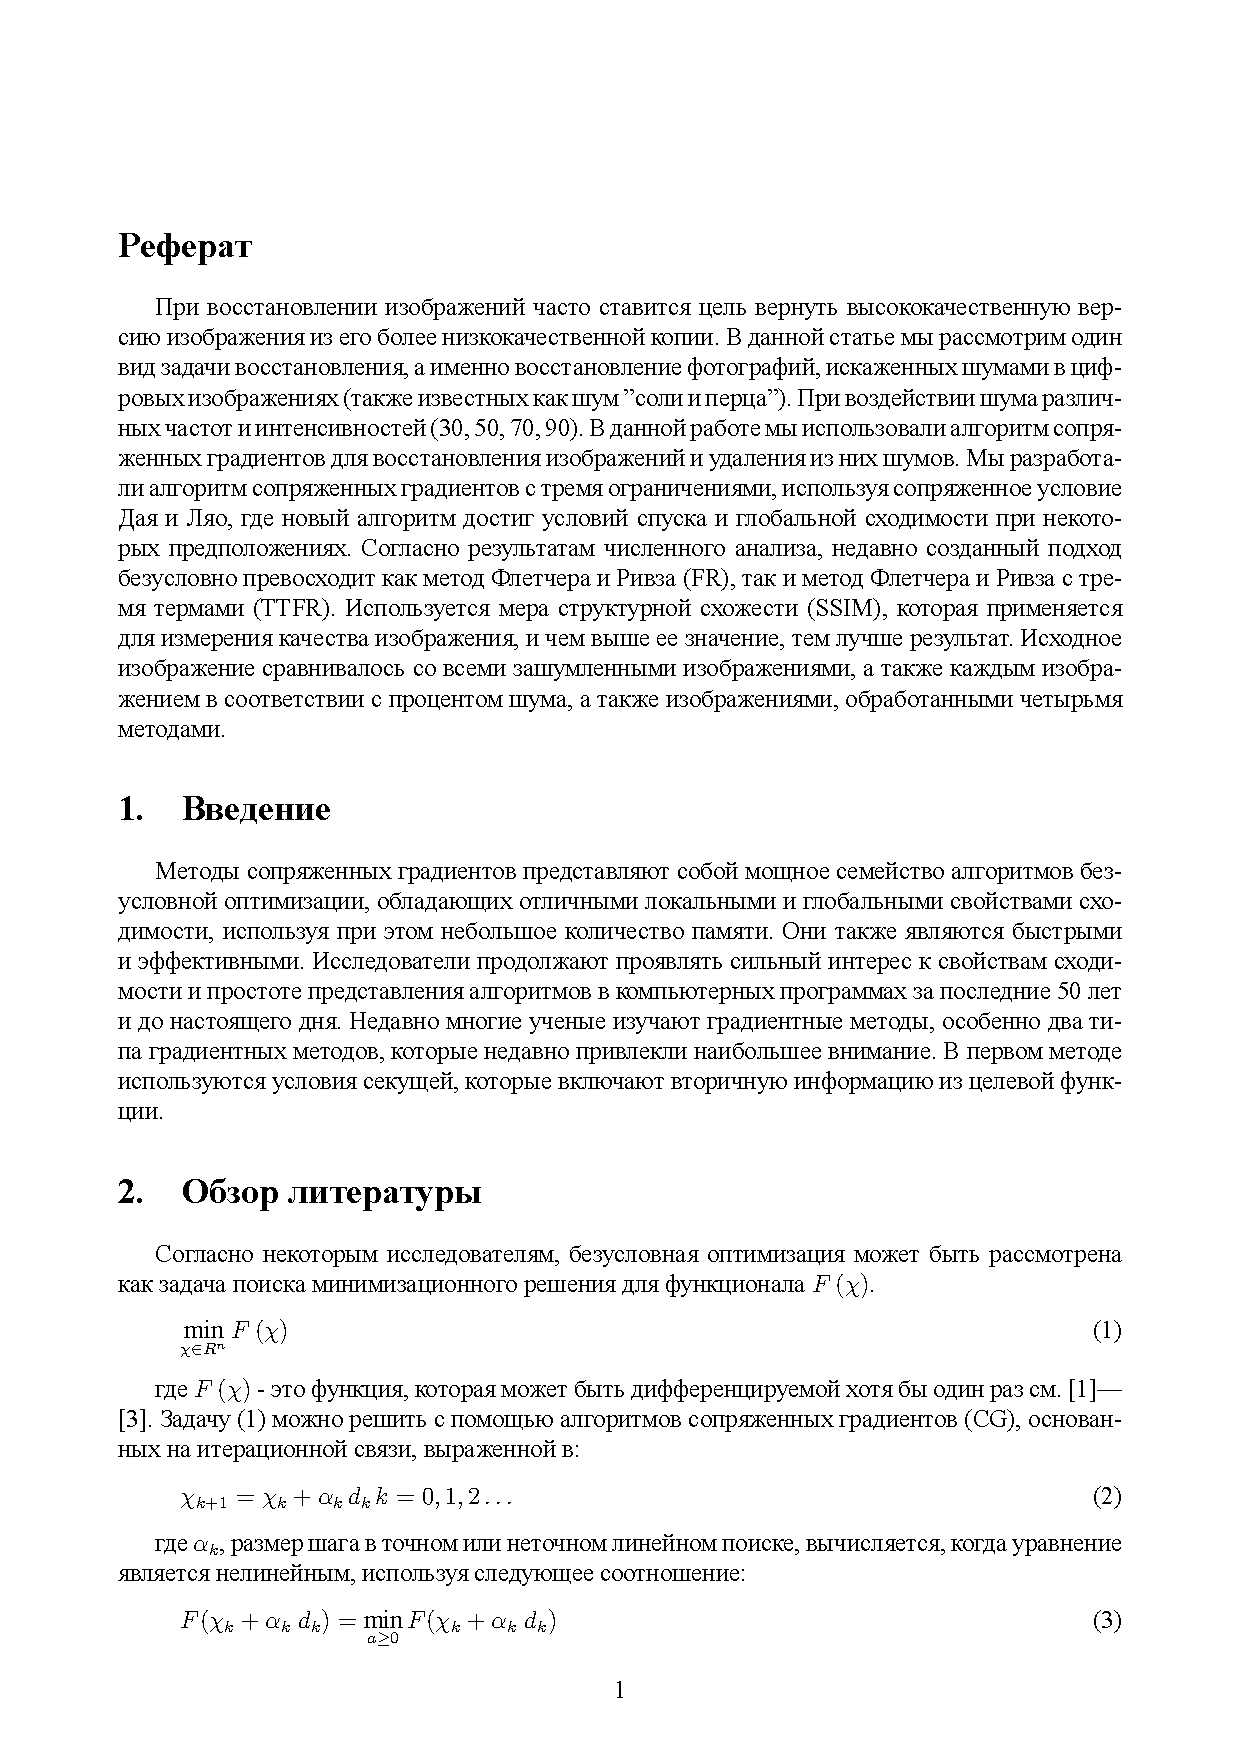
\includepdf[pages=1,offset=0 0, pagecommand={\subsection{Перевод статьи}\label{reference}\thispagestyle{plain}}
]{translation.pdf}

\includepdf[pages=2-,offset=0 0, pagecommand=\thispagestyle{plain}
]{translation.pdf}

\newpage
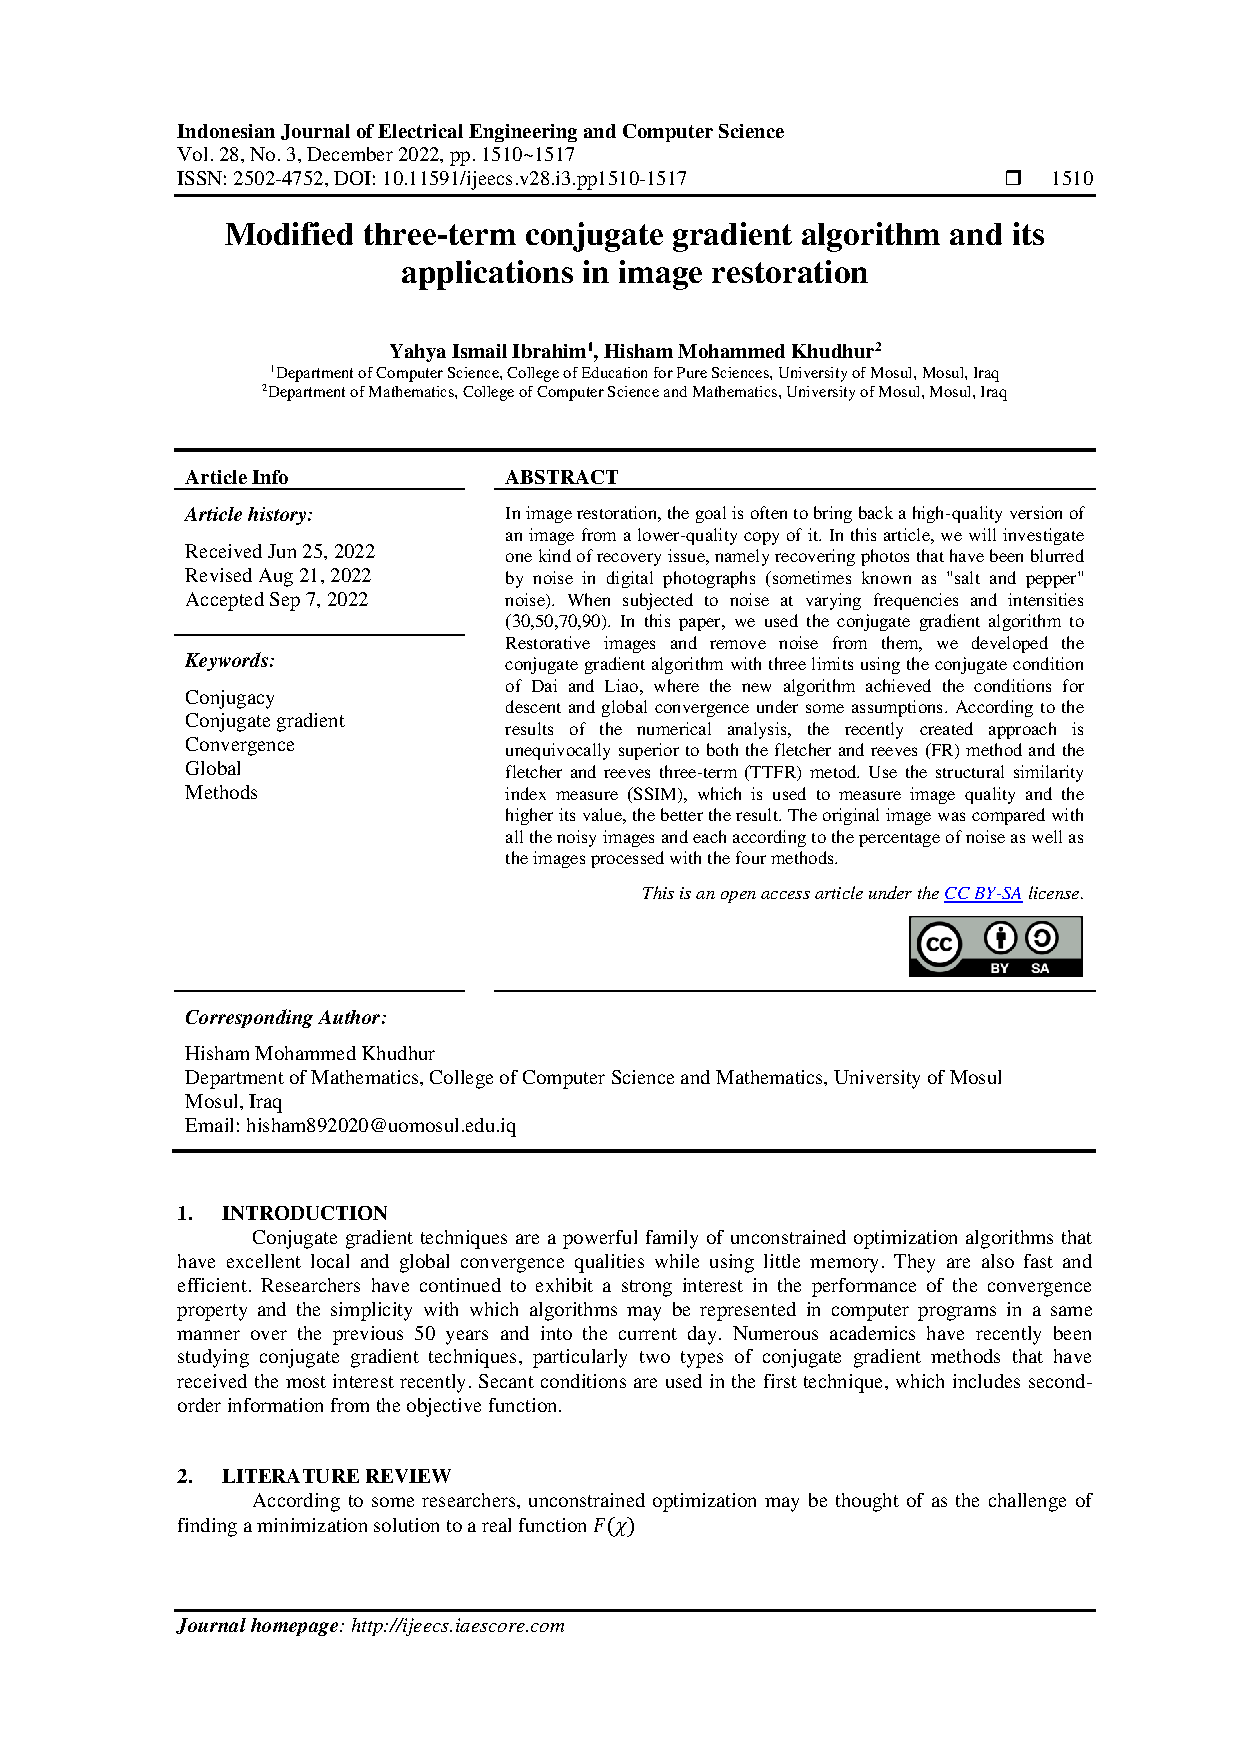
\includepdf[pages=1,offset=0 0, pagecommand={\subsection{Оригинальная статья}\label{reference}\thispagestyle{plain}}
]{Modified_three-term_conjugate_gradient_algorithm_a.pdf}

\includepdf[pages=2-,offset=0 0, pagecommand=\thispagestyle{plain}
]{Modified_three-term_conjugate_gradient_algorithm_a.pdf}

\end{document}
